\documentclass[12pt]{report}
\usepackage[left=2cm,right=2cm,top=2cm,bottom=2cm]{geometry} % page settings
\usepackage[dutch]{babel} % provides dutch alternatives for english text
\usepackage[utf8]{inputenc} % provides UTF-8 encoding
\usepackage{color} % more color options
\usepackage{enumitem} % options for enumerations
\usepackage{amsmath} % provides many mathematical environments & tools
\usepackage{graphicx} % for displaying images
\usepackage{array} % manipulating tables
\usepackage{amsfonts} % for math fonts
\usepackage[pageanchor=false]{hyperref}

%DOCUMENT INFORMATION
\title{Samenvatting Statistiek}
\author{Bert De Saffel}
\date{2017-2018}

% CUSTOM COMMANDS
\setlength{\parindent}{0mm}
\setlength{\extrarowheight}{5pt}
\graphicspath{{./img/}}
\newcommand{\todo}[1]{
{\color{red}\textunderscore{\textit{TODO: #1}}}
}
\newcommand{\exercise}[2]{
#1


\underline{Oplossing}

#2

\hrulefill
}
\newcommand{\example}[2]{
    \hrulefill
    
    Voorbeeld: #1
    
    #2
    
    \hrulefill
}

\begin{document}
\maketitle
\tableofcontents

\part{Herhaling Wiskunde A}
\chapter{Onbepaalde Integralen}
\section{Substitutiemethode}
%Stel $$\alpha = \varphi(t),\;dx = \varphi'(t)$$
%dan $$\int f(\varphi(t))\varphi'(t)dt = \int f(x) dx$$
\subsection{Voorbeeld 1}
\begin{equation*}
    \begin{split}
        \int \frac{t - 1}{t^2 + 4}dt & = \int \frac{t}{t^2 + 4}dt - \int \frac{dt}{t^2 + 4} \\
        \hbox{stel}\;\; &  u = t^2 + 4        \\
        \hbox{dan}\;\; & du = 2tdt \rightarrow dt = \frac{du}{2t} \\
        & \Rightarrow \int \frac{t}{2t u} du - \frac{1}{2}\arctan{\frac{t}{2}} \\
        & = \frac{1}{2}\int \frac{du}{u} - \frac{1}{2}\arctan{\frac{t}{2}}\\
        & = \frac{1}{2}\ln{u} - \frac{1}{2}\arctan{\frac{t}{2}} \\
        & = \frac{1}{2}\ln{t^2 + 4} - \frac{1}{2}\arctan{\frac{t}{2}} + C
    \end{split}
\end{equation*}
\subsection{Voorbeeld 2}
\begin{equation*}
    \begin{split}
        \int \frac{dy}{e^y + 4e^{-y}} & = \int \frac{e^y}{(e^y)^2 + 4} dy \\
        \hbox{stel}\;\; & u = e^y \\
        \hbox{dan}\;\; & du = e^ydy \rightarrow dy = \frac{du}{e^y}\\
        & \Rightarrow \int \frac{e^y}{e^y(u^2 + 4)} du \\
        & = \int \frac{du}{u^2 + 4} \\
        & = \frac{1}{2}\arctan{\frac{u}{2}}\\
        & = \frac{1}{2}\arctan{\frac{e^y}{2}} + C\\
    \end{split}
\end{equation*}
\section{Partieële integratie}
$$\int u\;dv = uv - \int v\;du$$
\subsection{Voorbeeld 1}
\begin{equation*}
    \begin{split}
        \int \ln(x) dx & = \int 1\cdot \ln(x) dx \\
        \hbox{stel}\; u & = ln(x) \; \hbox{en}\; v = \int dx\\
        \hbox{dan}\; du & = \frac{1}{x}dx \; \hbox{en}\; v = x\\
        & \Rightarrow x\ln(x) - \int x\cdot\frac{1}{x}dx\\
        & = x\ln(x) - \int dx\\
        & = x\ln(x) - x + C
    \end{split}
\end{equation*}
\subsection{Voorbeeld 2}
\begin{equation*}
    \begin{split}
        \int \frac{x + 1}{\cos^2(x)}dx & \\
        \hbox{stel}\; u & = x + 1 \; \hbox{en}\; v = \int \frac{1}{\cos^2(x)}dx\\
        \hbox{dan}\; du & = dx \; \hbox{en}\; v = \tan(x) \\
        & \Rightarrow (x+1)\tan(x) - \int \tan(x)dx  \\
        & = (x+1)\tan(x) + ln|cos(x)| + C  \\
    \end{split}
\end{equation*}
\subsection{Voorbeeld 3}
\begin{equation*}
    \begin{split}
        \int e^{-x}\sin(2x) & \\
        \hbox{stel}\; u & = \sin(2x) \; \hbox{en}\; v = \int e^{-x}dx\\
        \hbox{dan}\; du & = 2\cos(2x)dx \; \hbox{en}\; v = -e^{-x}\\
        & \Rightarrow= -e^{-x}\sin(2x) + 2 \int e^{-x}\cos(2x) dx\\
        \hbox{stel}\; u & = \cos(2x) \; \hbox{en}\; v = \int e^{-x}dx\\
        \hbox{dan}\; du & = -2\sin(2x)dx \; \hbox{en}\; v = -e^{-x}\\
        & \Rightarrow -e^{-x}\sin(2x) + 2\bigg[-e^{-x}\cos(2x)  - 2\int e^{-x}\sin(2x)dx   \bigg]\\
        & = -e^{-x}\sin(2x) - 2e^{-x}\cos(2x) -  4\int e^{-x}\sin(2x)dx\\
    \end{split}
\end{equation*}
Dus
\begin{equation*}
    \begin{split}
        & \int e^{-x}\sin(2x)  = -e^{-x}\sin(2x) - 2e^{-x}\cos(2x) -  4\int e^{-x}\sin(2x)dx \\
        \Leftrightarrow\; &  5\int e^{-x}\sin(2x) = -e^{-x}[\sin(2x) + 2\cos(2x)] \\
        \Leftrightarrow\; & \int e^{-x}\sin(2x) = \frac{-e^{-x}[\sin(2x) + 2\cos(2x)]}{5}
    \end{split}
\end{equation*}
\subsection{voorbeeld 4}
\begin{equation*}
    \begin{split}
        \int \sin^4(\theta) d\theta & = \int (\sin^2(\theta))^2 d\theta \\
        & = \int \bigg(\frac{1 - \cos(2\theta)}{2}\bigg)^2 d\theta \\
        & = \int \bigg(\frac{1}{4} - \frac{\cos(2\theta)}{2} + \frac{\cos^2(2\theta)}{4} \bigg)d\theta \\
        & = \int \frac{1}{4}d\theta - \int \frac{\cos(2\theta)}{2}d\theta + \int \frac{\cos^2(2\theta)}{4}d\theta \\
        & = \frac{\theta}{4} - \frac{\sin(2\theta)}{4} + \frac{\sin(4\theta) + 4\theta}{32} \\
        & = \frac{12\theta - 8\sin(2\theta) + \sin(4\theta)}{32} + C
    \end{split}
\end{equation*}
\part{Wiskunde B}
\chapter{Differentiaalvergelijking}
\section{Definities}
De algemene definitie is:
$$F(x, y, y', y'', ..., y^{(n)}) = 0$$
waarbij: \begin{itemize}
\item \textbf{x} een veranderlijke is.
\item \textbf{y} een functie van x is.
\item er minstens één afgeleide van y is.
\end{itemize}
\example{Differentiaalvergelijking}{
    $$ x + y + y' = 0$$
}

Een differentiaalvergelijking heeft een \textbf{orde} en een \textbf{graad}
\begin{itemize}
    \item \textbf{Orde}: Dit is de orde van de hoogste afgeleide dat voorkomt, dus \textit{n}.
    \item \textbf{Graad}: De graad \textit{r} bestaat niet altijd maar is wel altijd een strik positief geheel getal. De graad is de macht die behoort tot de afgeleide met de grootste orde. $y^{(n)^{r}}$
\end{itemize}
\example{Orde en graad}{
    \begin{center}
        \begin{tabular}{l | l | l}
            Differentiaalvergelijking                          & Orde & Graad \\
            \hline
            $y\ - 2y'^3 = yx$                                  & 2    & 1     \\
            $1 + (y'')^4 + 2y' + x(y''')^2 = sin(x)$           & 3    & 2     \\
            $(x - 1)(y'') - xy' + y = 0$                       & 2    & 1     \\
            $e^s\frac{d^3s}{dt^3} + (\frac{ds^2}{dt^2})^3 = 0$ & 3    & 1     \\
            $xy' + e^{y'} + y'' = 1$                           & 1    & /     \\
            \hline
            $\sin\sqrt {y'} = x + 2$                           & 1    & /     \\
            $\;\;\rightarrow y' = \arcsin^2(x+2)$              & 1    & 1     \\
            \hline
            $\sin y' = xy'^2$                                  & 1    & /     \\
            $\;\;\rightarrow y' = \arcsin(xy'^2)$              & 1    & /     \\
            \hline
            $y^{'3} + \frac{x}{y''} + y'' = 1$                 & 2    & ?     \\
            $\;\;\rightarrow y^{'3}y'' + x + (y'')^2 = 1$      & 2    & 2     
            
        \end{tabular}
    \end{center}
}
\section{Soorten oplossingen}
Tijdens het oplossen van een differentiaalvergelijking van de \textit{n}-de orde worden drie oplossingen onderscheden:
\begin{enumerate}
\item De \textbf{Algemene oplossing (AO)}: Verzameling van functies zodat de differentiaalvergelijking klopt. De algemene oplossing bevat \textit{n }onafhankelijke constanten. Deze constanten zijn getallen en geen functies.
\item De \textbf{Particuliere oplossing (PO)}: Dit is één van de krommen van de AO en is afhankelijk van de beginvoorwaarden van het probleem.
\item De \textbf{Singuliere oplossing (SO)}: Een oplossing die niet voldoet aan de AO maar wel een oplossing is voor de DVG.
\end{enumerate}
\example{Onafhankelijke variabelen:}
{
\begin{center}
    \begin{tabular}{l | l | l}
    AO & Onafh. C & Orde DVG \\
    \hline
    $y = C_1 + C_2x$ & 2 & 2 \\
    $y = C_1  - C_1^2x$ & 1 & 1 \\
    \hline
    $y = C_1(C_2 + C_3e^x)$ & ? & ? \\
    $\;\;\rightarrow C_1C_2 + C_1C_3e^x$ & ? & ? \\
    $\;\;\rightarrow a + be^x$ & 2 & 2 \\
    \hline
    $y = C_1 + \ln(C_2 x)$ & ? & ? \\
    $\;\;\rightarrow y = C_1 + \ln(C_2) + \ln(x)$ & ? & ? \\
    $\;\;\rightarrow y = a + \ln(x)$ & 1 & 1


    \end{tabular}
\end{center}
}
\example{Oef 1 AO en PO}{Gegeven een differentiaalvergelijking: $y'' + y = 0$
\begin{enumerate}
\item Toon aan dat $y = a\sin(x) + b\cos(x)$ de AO is.
\item Geef enkele PO's.
\end{enumerate}
Oplossing:
\begin{enumerate}
\item 
\begin{equation*}
\begin{split}
    y & = a\sin(x) + b\cos(x) \\
    y' & = a\cos(x) - b\sin(x) \\
    y'' & = -a\sin(x) - b\cos(x) 
\end{split}
\end{equation*}
Hieruit volgt:
\begin{gather*}
    y'' + y  = 0 \\
    -a\sin(x) - b\cos(x) + \sin(x) + b\cos(x)  = 0  \\
    \rightarrow \hbox{Het is een oplossing}
\end{gather*}
De differentiaalvergelijking heeft orde 2. De y-vergelijking bevat 2 onafhankelijke constanten en de y-vergelijking is een oplossing. Hierdoor is y de AO van de differentiaalvergelijking.
\item Enkele PO's:
\begin{equation*}
\begin{split}
y & = 0\\
y & = \sqrt{2}\sin(x) \\
y & = \sin(x) + \cos(x)
\end{split}
\end{equation*}
\end{enumerate}
}

\example{Oef 2 AO en PO}
{Gegeven een differentiaalvergelijking: $y'^2 - yy'+e^x$
\begin{enumerate}
\item Geef de orde en graad.
\item Is $y = \frac{1}{C} + Ce^x$ de AO?
\item Wat  voor soort oplossing is $y = 2\sqrt{e^x}$
\end{enumerate}
Oplossing:
\begin{enumerate}
\item 
De orde is 1 en de graad is 2.

\item 
$$y' = Ce^x$$
\begin{equation*}
\begin{split}
\rightarrow C^2(e^x)^2 - (\frac{1}{C} + Ce^x)Ce^x + e^x &  = 0 \\
\Leftrightarrow C^2e^{2x} - e^x - C^2e^{2x} + e^x &  = 0 \\
\Leftrightarrow C^2e^{2x} - e^x - C^2e^{2x} + e^x & = 0 \\
\Leftrightarrow 0 & =0
\end{split}
\end{equation*}
$$\rightarrow \hbox{Het is een oplossing}$$
Orde DVG = 1 = Onafhankelijke constanten van y

\item 
$$ y'  = 2 \cdot \frac{1}{2\sqrt{e^x}} \cdot e^x = \sqrt{e^x}$$
\begin{equation*}
\begin{split}
\rightarrow & y'^2 - yy'+e^x \\
\Leftrightarrow &  (\sqrt{e^x})^2 - 2\sqrt{e^x}\cdot\sqrt{e^x} + e^x  = 0 \\
\Leftrightarrow & e^x - 2e^x + e^x  = 0 \\
\Leftrightarrow & 0 = 0
\end{split}
\end{equation*}
Dit is een singuliere oplossing aangezien y niet overeenkomt met de AO, maar wel voldoet aan de DVG.

\end{enumerate}
}
\section{Bepalen van een DVG}
Indien een AO gegeven is met \textit{n} onafhankelijke constanten:
\begin{enumerate}
\item Controleer of de constanten werkelijk onafhankelijk zijn.
\item Leid de AO \textit{n} maal af.
\item Elimineer de \textit{n} constanten van de \textit{n + 1} bekomen vergelijkingen. De laatste vergelijking moet zeker gebruikt worden.
\item Controleer of de DVG van orde \textit{n} is.
\end{enumerate}

\example{Oef 1 bepalen van een DVG}
{
De algemene oplossing is $$y = C_1 + C_2x$$
\begin{enumerate}
\item Er zijn \textit{2} onafhankelijke constanten.
\item Er moet \textit{2} keer afgeleid worden:
$$
    \begin{cases}
    y    & = C_1 + C_2x \\
    y'   & = C_2 \\
    y''  & = 0 \\
    \end{cases}
$$
\item De constanten zijn al geëlimineerd. 
\item De DVG is $y'' = 0$ en heeft orde \textit{2}.

\end{enumerate}
}

\example{Oef 2 bepalen van een DVG}
{
Bepaal de DVG van: $$y = C_1 + C_2e^{-x} + C_3e^{3x}$$
\begin{enumerate}
\item Er zijn \textit{3} onafhankelijke constanten.
\item Er moet \textit{3} maal afgeleid worden.
    \[ 
    \begin{cases}
            y & = C_1 + C_2e^{-x} + C_3e^{3x} \\
    y'     & = -C_2e^{-x} + 3C_3e^{3x}     \\
    y'' & = C_2e^{-x} + 9C_3e^{3x}      \\
    y''' & = -C_2e^{-x} + 27C_3e^{3x}
    \end{cases}
    \]

\item 
Tel de 1ste afgeleide op met de 2de afgeleide en tel de 2de afgeleide op met de 3rde afgeleide
\[
    \begin{cases}
    y + y''    & = 3C_3e^{3x} + 9C_3e^{3x} = 12C_3e^{3x}  \\
    y'' + y''' & = 9C_3e^{3x} + 27C_3e^{3x} = 36C_3e^{3x}
    \end{cases}
\]
Vermenigvuldig de 1ste vergelijking met 3 en trek hiervan de 2de vergelijking af.

$$3(y + y'') - y'' - y''' = 3(12C_3e^{3x}) - 36C_3e^{3x} = 0$$
$$\rightarrow y''' - 2y'' - 3y' = 0$$
\item
De orde van deze DVG is \textit{3}

\end{enumerate}
}

\example{Oef 3 bepalen van een DVG}
{
Bepaal de DVG van alle cirkels met middelpunt y = -x.
\begin{enumerate}
\item Eerst moet de AO gevonden worden. Het middelpunt van elke cirkel kan gegeven worden met $m(a, -a).$
    Hieruit volgt de algemene vergelijking van een cirkel: $$(x - a)^2 + (y + a)^2 = R^2$$
    Er zijn \textit{2} onafhankelijke constanten (a en R).
\item Er moet \textit{2} maal (impliciet) afgeleid worden.
\[
    \begin{cases}
    (x - a)^2 + (y + a)^2 = R^2 \\
    \frac{dy}{dx} : (x-a) + y'(y+a) = 0 \\
    \frac{d^2y}{dx^2} : 1 + y''(y + a) + y'^2 = 0
    \end{cases}
\]
\item
    Vorm $\frac{dy}{dx}$ om naar $a$:
    $$a = \frac{-x - yy'}{y' - 1}$$
    Substitueer deze $a$ in $\frac{d^2y}{dx^2}$:
    $$1 + y''(y + (\frac{-x - yy'}{y' - 1})) + y'^2 = 0$$
    $$\rightarrow 1 + y''(y + (\frac{x + yy'}{-y' + 1})) + y'^2 = 0$$
    $$\rightarrow y''(x + y) - y'^3 + y'^2 - y' + 1 = 0$$
\item Orde van de DVG = \textit{2}  = Aantal onafhankelijke constanten.
\end{enumerate}
}
\section{Oplossen van een lineaire DVG van orde n met constante reële coëfficiënten}
\begin{equation*}
 \begin{split}
		  & y''' - y''\sin t + ty = t^2 \\
  \Leftrightarrow & D^3y - D^2y\sin t + ty = t^2 \\
  \Leftrightarrow & (D^3 - D^2\sin t + t)y = t^2 \\
  \Leftrightarrow & L(d)y = g(t) \\
  \Leftrightarrow & \hbox{met} L(d) = \sum_{i = 0}^{n} a_iD^i \qquad ,a_i \in \mathbb{R}
 \end{split}
\end{equation*}
Een lineaire DVG is een DVG waarbij alle coëfficiënten van alle afgeleiden enkel voorkomen als eerste macht.
\subsection{Particuliere oplossing}
De particuliere oplossing kan slechts bepaald worden indien alle beginvoorwaarden ($y(0), y'(0),...,y^{(n-1)}(0)$) gekend zijn.
\subsection{Algemene oplossing}
Indien de beginvoorwaarden niet gekend zijn moeten $y(0),y'(0)...y^{(n-1)}(0)$ respectievelijk gelijkgesteld worden aan $C_1, C_2, ..., C_n$

\example{
  Bepaal de PO van $y'' + y = g(t)$ indien $y(0) = 0$, $y'(0) = 1$ en 
  $$
    g(t) = \begin{cases}
	      0 & t < 1 \\
	      e^{-t} & t > 1
	   \end{cases}
  $$
}{
  \begin{equation*}
   \begin{split}
                   & L(d)y = g(t) \\
   \Leftrightarrow & (D^2 + 1)y = g(t) \\
   \Leftrightarrow & (D^2 + 1)y = e^{-t}H(t - 1) \\
   \mathcal{L}\{LL\}(s) & = \mathcal{L}\{y'' + y\}(s) \\
                        & = s^2Y - sy(0^{+}) + y'(0^{+}) + Y \\
                        & = s^2Y - 1 + Y \\
   \mathcal{L}\{RL\}(s) & = \mathcal{L}\{e^{-t}H(t - 1\}(s) \\
                        & = \mathcal{L}\{e^{-(t - 1) - 1}H(t - 1)\}(s) \\
                        & = e^{-1}\mathcal{L}\{e^{-(t - 1)}H(t - 1)\}(s) \\
                        & = e^{-1}e^{-s}\mathcal{L}\{e^{-t}\}(s) \\
                        & = e^{-1}e^{-s}\frac{1}{s + 1} \\
                        & = \frac{e^{-(s + 1)}}{s + 1} \\
   \hbox{dus} \\
   \Leftrightarrow & s^2Y - 1 + Y = \frac{e^{-(s + 1)}}{s + 1} \\
   \Leftrightarrow & Y(s^2 + 1) = 1 + \frac{e^{-(s + 1)}}{s+1} \\
   \Leftrightarrow & Y = \frac{1}{s^2 + 1} + \frac{e^{-(s+1)}}{(s+1)(s^2+1)}     \\
   \Leftrightarrow & \mathcal{L}^{-1}\{Y\}(t) = \mathcal{L}^{-1}\bigg\{\frac{1}{s^2 + 1} + \frac{e^{-(s+1)}}{(s+1)(s^2+1)}\bigg\}(t) \\
   \Leftrightarrow & y(t) = \sin t +e^{-1}f(t - 1)H(t - 1) \\
	   \hbox{met}\; f(t) & = \mathcal{L}^{-1}\bigg\{\frac{1}{(s + 1)(s^2 + 1)}\bigg\}(t) \\
			     & = \frac{1}{2}\mathcal{L}^{-1}\bigg\{\frac{1}{s + 1} - \frac{s - 2}{s^2 + 1}\bigg\}(t) \\
			     & = \frac{1}{2}\bigg[e^{-t} - (\cos t + \sin t)\bigg] \\
	    \hbox{antwoord: }\; y(t)  & = \sin t + \frac{1}{2}\bigg(e^{-t} - e^{-1}\cos (t - 1) + e^{-1} \sin (t - 1) \bigg)H(t - 1)
   \end{split}
  \end{equation*}

}
\example{
  Bepaal de PO van $y'' + y = \delta\big(t - \frac{\pi}{2}\big)$ indien $y(\frac{\pi}{4}) = 0$, $y'(\frac{\pi}{4}) = 0$
}{
  $y(0^+) = C_1$, $y'(0^+) = C_2$
  \begin{equation*}
   \begin{split}
    \mathcal{L}\{LL\}(s) & = \mathcal{L}\{y'' + y\}(s) \\
			 & = s^2Y - sC_1 - C_2 + Y \\
    \mathcal{L}\{RL\}(s) & = \mathcal{L}\bigg\{\delta\big(t - \frac{\pi}{4}\bigg)\bigg\}(s) \\
                         & = \int_0^{+\infty}\delta\big(t - \frac{\pi}{4}\big)e^{-st} \; dt \\
                         & = e^{-\frac{\pi}{2}s}
   \end{split}
  \end{equation*}

}


\chapter{Laplacetransformatie}
\section{De Heaviside functie}
De Heaviside functie heeft als voorschrift:
$$H(t - a) = 
\begin{cases}
0 \;\; t < a \\
1 \;\; t > a
\end{cases}$$

\example{Teken over $x=[-3,4]$ de functie $y = 2H(t + 2) - tH(t) + (t+t^2)H(t-2)$}
{
Er zijn veranderingen bij $t = -2, t = 0$ en $t = 2$.

    \begin{tabular}{l | l}
    $2\cdot(0) - t\cdot(0) + (t+t^2)\cdot(0) = 0$ & $t < -2$\\
    $2\cdot(1) - t\cdot(0) + (t+t^2)\cdot(0) = 2$ & $-2 < t < 0$  \\
    $2\cdot(1) - t\cdot(1) + (t+t^2)\cdot(0) = 2 - t$ & $0 < t < 2$\\
    $2\cdot(1) - t\cdot(1) + (t+t^2)\cdot(1) = 2 + t^2$ & $t > 2$\\
    \end{tabular}
\todo{graph}
}
\example{Schrijf met behulp van de Heaviside functie de stuksgewijze continue functie:
$$f(t) = \begin{cases}
        e^t & t < 2 \\
        1 - e^t & 2 < t < 3 \\
        t^2 & 3 < t < 5 \\
        t - 25 & t > 5
        \end{cases}
$$}{
\begin{equation*}
\begin{split}
    f(t) & = e^t + H(t-2)(-e^t + 1 - e^t) + H(t-3)(-1 + e^t + t^2) + H(t - 5)(-t^2 + t - 25) \\
    & = e^t + (1-2e^t)H(t-2) + (t^2+e^t-1)H(t-3) - (t^2-t+25)H(t-5)
\end{split}
\end{equation*}
}

\section{De Dirac delta-'functie'}
De Dirac delta-functie heeft als voorschrift:
$$
\begin{cases}
\delta(t - a) = 0 & t \neq a \\
\int_{a - \epsilon_1}^{a + \epsilon_2} \delta(t - a) \; dt = 1 & \forall \epsilon_1, \epsilon_2 > 0 
\end{cases}
$$
De meetkundige betekenis: We nemen de limiet van $\delta^a_{\epsilon_1,\epsilon_2}(t)$ voor $\epsilon_1,\epsilon_2 \rightarrow 0$
$$\delta^a_{\epsilon_1,\epsilon_2}(t) = \begin{cases}
                                        0 & \forall t < a - \epsilon_1 \; \hbox{of} \; t > a + \epsilon_2 \\
                                        \frac{1}{\epsilon_1 + \epsilon_2} & \forall \in ]a - \epsilon_1, a + \epsilon_2[
                                        \end{cases}
$$
Het nut van de dirac functie is om bepaalde integralen op te lossen. Meer bepaald de integralen van de vorm:
$$\int_{0}^{+\infty} f(t) \delta(t- a)\;dt = f(a)$$
De ondergrens 0 mag ook vervangen worden door $-\infty$ aangezien elke functie causaal is binnen het domein van Laplace.

De afgeleide van de Heaveiside functie is gelijk aan de delta functie:
$$\frac{d}{dt}H(t-a) = \delta(t - a)$$
\example{$$\int_{0}^{+\infty} (2\sin t - 1) \delta(t - \frac{3\pi}{2}) \; dt$$}{
In dit geval is $f(t) = (2\sin t - 1)$ en $\delta(t - a) = \delta(t - \frac{3\pi}{2})$
We kunnen dus makkelijk deze integraal oplossen door gebruik te maken van de definitie:
\begin{equation*}
\begin{split}
\int_{0}^{+\infty} f(t) \delta(t- a)\;dt & = \int_{0}^{+\infty} (2\sin t - 1) \delta(t - \frac{3\pi}{2}) \; dt \\
                                        & = f(\frac{3\pi}{2}) - 1  \\
                                        & = 2\sin \bigg(\frac{3\pi}{2}\bigg) - 1 \\
                                        & = -2 - 1 \\
                                        & = - 3
\end{split}
\end{equation*}
}
\section{Causale functie}
Een causale functie is een functie $f$ waarvoor $f(t) = 0$ voor elke $t < 0$.
Om een willekeurige functie causaal te maken voeg je de Heaviside functie achteraan toe.
$$f(t) \rightarrow f(t)H(t)$$
Dit zorgt ervoor dat voor elke $t < 0$ dat $f(t) = 0$. De afspraak is dat deze Heaviside functie nu achter elke functie komt zonder dat we deze nog schrijven. Elke functie is vanaf nu dus causaal.

\example{Teken de causale functie $f(t)$ gedefinieerd als: -2 indien t $<$ 1 en 2 als t $>$ 1. Schrijf ze ook met behulp van de Heaviside functie}{
De functie kan omschreven worden als:
$$f(t) = \begin{cases}
        0 & t < 0 \\
        -2 & 0 < t < 1 \\
        2 & t > 1
        \end{cases}
$$
Omgevormd met de Heaviside-functie:
\begin{equation*}
\begin{split}
f(t) & = H(t)(-0 + (-2)) + H(t -  1)(-2 +2) \\
    & = -2H(t) + 4H(t - 1)
\end{split}
\end{equation*}
Tekening:
\todo{graph}
}
\section{Exponentiële orde}
Een functie is van exponentiële orde indien $\exists M, a \in R$ zodat $|f(t)| < Me^{at}, \forall t > N$ en met a het minimum van de waarden waarvoor dit geldt. Indien waar is $f(t)$ van exponentiële orde a.
Soms is het gemakkelijker te bewijzen via:
$$\lim_{t \to +\infty} \frac{|f(t)|}{e^{at}} \in R$$
\example{Bepaal de exponentiële orde van $\sin t$}{
\begin{equation*}
\begin{split}
                & |\sin t| \leq 1 \\
\Leftrightarrow & |\sin t| < 1.1 \hbox{(willekeurige waarde)} \\
\Leftrightarrow & |\sin t| < 1.1e^{at}
\end{split}
\end{equation*}
Hieruit kan afgeleid worden dat a = 0 en de exponentiële orde is dus ook 0.
}
\example{Bepaal de exponentiële orde van $(1 + 2t)e^{-t}$}{
Bij deze opgave maken we gebruik van de limietstelling.
\begin{equation*}
\begin{split}
\lim_{t \to +\infty} \frac{|f(t)|}{e^{at}} & = \lim_{t \to +\infty} \frac{|(1 + 2t)e^{-t}|}{e^{at}} \\
                                            & = \lim_{t \to +\infty} \frac{(1 + 2t)e^{-t}}{e^{at}} \\
                                            & = \lim_{t \to +\infty} \frac{1 + 2t}{e^{at}e^{t}} \\
                                            & = \lim_{t \to +\infty} \frac{1 + 2t}{e^{t(a +1)}} 
\end{split}
\end{equation*}
We moeten een onderscheid maak tussen 2 gevallen:
\begin{itemize}
\item $a + 1 < 0 \rightarrow e^{-\infty} = 0 \rightarrow \frac{+\infty}{0} \rightarrow \; \hbox{onbepaald}$
\item $a + 1 > 0 \rightarrow e^{+\infty} = \infty \rightarrow \frac{+\infty}{+\infty} \rightarrow \; \hbox{L'Hopital}$
\end{itemize}
We maken enkel gebruik van het tweede geval en passen dus L'hopital toe.
\begin{equation*}
\begin{split}
\lim_{t \to +\infty} \frac{1 + 2t}{e^{t(a +1)}} & = \lim_{t \to +\infty} \frac{2}{e^{t(a +1)}(a+1)} \\
                                                & = \frac{2}{+\infty} = 0 \in R
\end{split}
\end{equation*}
Aangezien het een reëele uitkomst is kan a uit de uitdrukking $a + 1 > 0$ afgeleid worden.
$$\forall a, a > -1$$
De exponentiële orde is dus -1.
}
\section{De Laplacetransformatie}
Definitie: Stel $f(t)$ causuaal dan is de laplacetransformatie van $f(t)$ een functie die een complex getal $s$ afbeeldt op 
$$\mathcal{L}\{f(t)\}(s) = F(s) = \int_{0}^{+\infty}f(t)e^{-st}\;dt, s \in \mathbb{C}$$
Een voorbeeld uit het formularium:
$$\mathcal{L}\{\sin t\}(s) = \frac{1}{1 + s^2}$$
De letter s kan eender welk complex getal zijn:
$$\mathcal{L}\{\sin t\}(2) = \frac{1}{1 + 4}$$
Indien er een imaginaire eenheid is verandert de definitie minimaal:
$$\mathcal{L}\{\sin t\}(3 + 2j) = \int_{0}^{+\infty}|f(t)e^{-st}|\;dt$$
Het argument tussen de $| ... |$ is NIET de absolute waarde, maar de MODULUS van het complexe getal, te berekenen via $\sqrt{x^2 + y^2}$ indien het complexe getal gedefinieerd wordt als $s = x + yj$ (wat vanaf nu als definitie gebruikt wordt voor een complex getal).
\subsection{Opmerkingen}
\begin{enumerate}
\item $$|f(t)e^{-st}| = |f(t)|e^{-xt}, \; s = x+yj$$
want
\begin{equation*}
\begin{split}
|f(t)e^{-st}| & = |f(t)e^{-(x + yj)t}| \\
                & = |f(t)|\cdot|e^{-(xt + yjt)}| \\
                & = |f(t)|\cdot|e^{-xt} \cdot e^{-yjt}| \\
                & = |f(t)|\cdot|e^{-xt}|\cdot|e^{-yjt}| \\
                & = |f(t)|\cdot e^{-xt}\cdot|\cos(-yt) + j\sin(-yt)| \\
                & = |f(t)|e^{-xt}\sqrt{\cos^2{(-yt)} + \sin^2{(-yt)}} \\
                & = |f(t)|e^{-xt}
\end{split}
\end{equation*}
\item 
$$\mathcal{L}\{af(t) + bg(t)\}(s) = a\mathcal{L}\{f(t)\}(s) + b\mathcal{L}\{g(t)\}(s)$$
De Laplace van een som is gelijk aan de som van een Laplace.
\end{enumerate}
\subsection{Laplacegetransformeerde van enkele basisfuncties}
\begin{itemize}
\item $$\mathcal{L}\{e^{at}\}(s) = \frac{1}{s - a}$$
Bewijs:
\begin{equation*}
\begin{split}
\mathcal{L}\{e^{at}\}(s) & = \int_{0}^{+\infty}e^{at}e^{-st} \; dt \\
                            & = \int_{0}^{+\infty} e^{t(a - s)} \; dt \\
                            & = \frac{e^t{a - s)}}{a - s}\bigg|_{0}^{+\infty} \\
                            & = \frac{1}{a - s}\bigg(\lim_{t \to +\infty}e^{t(a - s)} - 1\bigg)                         
\end{split}
\end{equation*}
Uitwerking van de limiet:
\begin{equation*}
\begin{split}
    \lim_{t \to +\infty}e^{t(a - s)} & = \lim_{t \to +\infty}|e^{at - st)} | \\
                                    & = \lim_{t \to +\infty}|e^{at - (x + yj)t}| \\
                                    & = \lim_{t \to +\infty}|e^{at - xt}\cdot e^{-yjt}| \\
                                    & = \lim_{t \to +\infty}|e^{at - xt}|\cdot |e^{-yjt}| \\
                                    & = \lim_{t \to +\infty}|e^{at - xt}|\cdot |\cos(-yt) + j\sin(-yt)| \\
                                    & = \lim_{t \to +\infty}e^{at - xt}\cdot \sqrt{\cos^2(-yt) + \sin^2(-yt)} \\
                                    & = \lim_{t \to +\infty}e^{at - xt} = e^{-\infty} = 0
\end{split}
\end{equation*}
Deze uitkomst in de oorspronkelijke vergelijking steken:
$$\frac{1}{a - s}(0 - 1) = \frac{1}{s - a}$$ 

\item $$\mathcal{L}\{\sin \omega t\}(s) = \frac{\omega}{\omega^2 + s^2} \qquad  \hbox{en} \qquad  \mathcal{L}\{\cos \omega t\}(s) = \frac{s}{\omega^2 + s^2}$$
Bewijs: We vertrekken van de uitkomst van vorig bewijs. Beschouw $a = wj$
\begin{equation*}
\begin{split}
\mathcal{L}\{e^{wjt}\}(s) & = \frac{1}{s - wj} \\
                            & = \frac{1}{s - wj} \cdot \frac{s + wj}{s + wj} \\
                & = \frac{s + wj}{s^2 + w^2}\\
                & = \mathcal{L}\{\cos (\omega t) + j\sin(\omega t)\}(s) \\
                & = \mathcal{L}\{\cos (\omega t)\}(s) + \mathcal{L}\{j\sin(\omega t) \}(s) \\
                & = \frac{s}{s^2 + w^2} + \frac{w}{s^2 + w^2}j \\ 
\end{split}
\end{equation*}
dus $$\mathcal{L}\{\cos \omega t\}(s) = \frac{s}{\omega^2 + s^2} \qquad  \hbox{en} \qquad  \mathcal{L}\{\sin \omega t\}(s) = \frac{\omega}{\omega^2 + s^2}$$

\item 
$$\mathcal{L}\{\delta(t)\}(s) = 1$$
Bewijs:
\begin{equation*}
\begin{split}
    \mathcal{L}\{\delta(t)\}(s) & = \mathcal{L}\{\delta(t - 0)\}(s) \\
                & = \int_{0}^{+\infty}\delta(t - 0)e^{-st}\;dt \\
                & = f(0) = e^{-s\cdot0} = e^{0} = 1
\end{split}
\end{equation*}
\end{itemize}
\example{Bepaal het laplacebeeld van $\cos{(2t - 1)}$}{
\begin{equation*}
\begin{split}
\mathcal{L}\{\cos(2t - 1)\}(s) & = \mathcal{L}\{\cos(2t)\cos( 1 )+ \sin(2t)\sin (1)\}(s) \\
                & = \cos (1) \mathcal{L}\{\cos 2t\}(s) + \sin (1 )\mathcal{L}\{\sin 2t\}(s)\\
                & = \cos (1) \frac{s}{s^2 + 4} + \sin (1) \frac{2}{s^2 + 4} \\
                & = \frac{s\cos(1)}{s^2 + 4} + \frac{2\sin(1)}{s^2 + 4}
\end{split}
\end{equation*}
}
\example{Bepaal het laplacebeeld van $\sinh(4t) - 3\cos{(\frac{t}{3})}$}
{
\begin{equation*}
\begin{split}
\mathcal{L}\bigg\{\ \sinh(4t) - 3\cos{\bigg(\frac{t}{3}\bigg)} \bigg\}(s) & = \mathcal{L}\bigg\{\ \frac{e^{4t} - e^{-4t}}{2} - 3\cos{\bigg(\frac{t}{3}\bigg)} \bigg\}(s) \\
& = \mathcal{L}\bigg\{\ \frac{e^{4t} - e^{-4t}}{2}\bigg\}(s) - 3\mathcal{L}\bigg\{\cos{\bigg(\frac{t}{3}\bigg)} \bigg\}(s) \\
& = \frac{1}{2}\bigg(\frac{1}{s - 4} - \frac{1}{s + 4}\bigg) - 3\frac{s}{s^2 + \frac{1}{9}} \\
& = \frac{1}{2}\bigg(\frac{1}{s - 4} - \frac{1}{s + 4}\bigg) - \frac{27s}{9s^2 + 1}
\end{split}
\end{equation*}
}
\example{Bepaal het laplacebeeld van $\delta(t - \frac{\pi}{2})\cos(4t)e^{2t}$}{
\begin{equation*}
\begin{split}
\mathcal{L}\bigg\{\delta\bigg(t - \frac{\pi}{2}\bigg)\cos(4t)e^{2t}\bigg\}(s) & = \int_{0}^{+\infty}\cos(4t)e^{2t}\delta\bigg(t - \frac{\pi}{2}\bigg)e^{-st} \; dt \\
& = f\bigg(\frac{\pi}{2}\bigg) \\
& = \cos\bigg(4 \cdot \frac{\pi}{2}\bigg)e^{2\cdot\frac{\pi}{2}}e^{-s\cdot\frac{\pi}{2}} \\
& = \cos(2\pi)e^{\pi}e^{-\frac{s\pi}{2}}\\
& = e^{\pi}e^{-\frac{s\pi}{2}}
\end{split}
\end{equation*}

}
\subsection{Translatie naar rechts}
Definitie:
$$\mathcal{L}\{f(t - a)H(t - a)\}(s) = e^{-as}F(s) \qquad a > 0$$
Bewijs:
\begin{equation*}
\begin{split}
\mathcal{L}\{f(t - a)H(t - a)\}(s) & = \int_{0}^{+\infty}f(t - a)H(t - a)e^{-st} \; dt \\
                                    & = \int_{0}^{a}f(t - a)H(t - a)e^{-st} \; dt + \int_{a}^{+\infty}f(t - a)H(t - a)e^{-st} \; dt \\
                                    & = 0 +\int_{a}^{+\infty}f(t - a)H(t - a)e^{-st} \; dt \\
                                    & = \int_{a}^{+\infty}f(t - a)H(t - a)e^{-st} \; dt \\
                                    \hbox{stel}\quad u & = t - a \\
                                    \hbox{dan}\quad du & = dt \\    
                                    & = \int_{0}^{+\infty}f(u)e^{-s(u + a)} \; du \\
                                    & = \int_{0}^{+\infty}f(u)e^{-su}e^{-sa} \; du \\
                                    & = e^{-sa}\int_{0}^{+\infty}f(u)e^{-su} \; du \\
                                    & = e^{-sa}\mathcal{L}\{f(t)\}(s) \\
                                    & = e^{-as}F(s)
\end{split}
\end{equation*}
\example{Bepaal het laplacebeeld van $f(t) = (t^2 - 1)H(t - 1) - \sin(3t)H(t - \pi)$}
{
\begin{equation*}
\begin{split}
\mathcal{L}\{f(t)\} & = \mathcal{L}\{(t^2 - 1)H(t - 1)\}(s) - \mathcal{L}\{\sin(3t)H(t-\pi)\}(s)
\end{split}
\end{equation*}
We werken beide laplacetransformaties afzonderlijk uit:
\begin{equation*}
\begin{split}
%t^2 - 1 = (t - 1)^2 + 2t - 2 = (t - 1)^2 + 2(t - 1)%
\mathcal{L}\{(t^2 - 1)H(t - 1)\}(s) & = \mathcal{L}\{[(t-1)^2 + 2(t - 1)]H(t - 1)\}(s)\\
                                    & = e^{-as}\mathcal{L}\{t^2 + 2t\}(s) \\
                                    & = e^{-s}\bigg(\frac{2!}{s^3} + 2\frac{1!}{s^2}\bigg) \\
                                    & = e^{-s}\bigg(\frac{2}{s^3} + \frac{2}{s^2}\bigg)\\
                                    & = e^{-s}\bigg(\frac{2(1 + s)}{s^3}\bigg)
\end{split}
\end{equation*}
\begin{equation*}
\begin{split}
    %sin 3t = sin(3(t - \pi)) + 3\pi) = sin(3(t - \pi) + \pi) = -sin(3(t-\pi))%
\mathcal{L}\{\sin(3t)H(t-\pi)\}(s) & =  \mathcal{L}\{-\sin(3(t - \pi))H(t-\pi)\}(s) \\
                                    & = -e^{-\pi s}\mathcal{L}\{\sin (3t)\}(s) \\
                                    & = -e^{-\pi s}\frac{3}{s^2 + 9} \\
                                    & = -\frac{3e^{-\pi s}}{s^2 + 9}
\end{split}
\end{equation*}
Het resultaat wordt:
\begin{equation*}
\begin{split}
\mathcal{L}\{f(t)\} & = \mathcal{L}\{(t^2 - 1)H(t - 1)\}(s) - \mathcal{L}\{\sin(3t)H(t-\pi)\}(s) \\
                    & = e^{-s}\bigg(\frac{2(1 + s)}{s^3}\bigg) - \bigg(-\frac{3e^{-\pi s}}{s^2 + 9}\bigg) \\
                    & = e^{-s}\bigg(\frac{2(1 + s)}{s^3}\bigg) +\frac{3e^{-\pi s}}{s^2 + 9}
\end{split}
\end{equation*}
}
\subsection{Dempingsfunctie}
Definitie:
$$\mathcal{L}\{e^{-at}f(t)\}(s) = F(s + a)$$
\example{Bepaal het laplacebeeld van $f(t) = t(t^3 - 1)^2e^{-t} + \sin(\sqrt{3}t)e^{2t}$}
{
\begin{equation*}
\begin{split}
\mathcal{L}\{f(t)\}(s) = \mathcal{L}\{t(t^3 - 1)^2e^{-t}\}(s) + \mathcal{L}\{\sin(\sqrt{3}t)e^{2t}\}(s)
\end{split}
\end{equation*}
Ook hier beschouwen we beide laplacetransformaties apart.
\begin{equation*}
\begin{split}
\mathcal{L}\{t(t^3 - 1)^2e^{-t}\}(s) & = \mathcal{L}\{(t^7 - 2t^4 + t)e^{-t}\}(s) \\
                                    & = \mathcal{L}\{t^7 - 2t^4 + t\}(s + 1) \\
                                    & = \frac{7!}{(s + 1)^8} - \frac{2 \cdot 4!}{(s + 1)^5} + \frac{1!}{(s + 1)^2} \\
                                    & = \frac{7!}{(s + 1)^8} - \frac{48}{(s + 1)^5} + \frac{1}{s^2 + 2s + 1}
\end{split}
\end{equation*}
\begin{equation*}
\begin{split}
\mathcal{L}\{\sin(\sqrt{3}t)e^{2t}\}(s) & = \mathcal{L}\{\sin(\sqrt{3}t)\}(s - 2) \\
                                        & = \frac{\sqrt{3}}{(s - 2)^2 + 3} \\
                                        & = \frac{\sqrt{3}}{s^2 -2s + 7}
\end{split}
\end{equation*}
Het resultaat wordt:
\begin{equation*}
\begin{split}
\mathcal{L}\{f(t)\}(s) & = \mathcal{L}\{t(t^3 - 1)^2e^{-t}\}(s) + \mathcal{L}\{\sin(\sqrt{3}t)e^{2t}\}(s) \\
                        & = \frac{7!}{(s + 1)^8} - \frac{48}{(s + 1)^5} + \frac{1}{s^2 + 2s + 1} + \frac{\sqrt{3}}{s^2 -2s + 7}
\end{split}
\end{equation*}
}
\subsection{Schaalwijziging}
Definitie:
$$\mathcal{L}\{f(at)\}(s) = \frac{1}{a}F(\frac{s}{a})$$
Bewijs:
\begin{equation*}
 \begin{split}
  \mathcal{L}\{f(at)\}(s) & = \int_{0}^{+\infty}f(at)e^{-st}\;dt \\
                    \hbox{stel}\; u & = at \\
                    \hbox{dan}\; du & = adt \\
                          & =  \int_{0}^{+\infty}f(u)e^{-s\frac{u}{a}}\;\frac{du}{a} \\
                          & =  \frac{1}{a}\int_{0}^{+\infty}f(u)e^{-\frac{s}{a}u}\;du \\
                          & =  \frac{1}{a}\mathcal{L}\{f(u)\}(\frac{s}{a}) \\
                          & =  \frac{1}{a}F(\frac{s}{a})
 \end{split}
\end{equation*}
\example{Gegeven $\mathcal{L}\{\sin t\}(s) = \frac{1}{s^2 + 1}$. Bepaal $\mathcal{L}\{\sin \omega t\}(s)$}
{
\begin{equation*}
 \begin{split}
  \mathcal{L}\{f(\omega t)\}(s) & = \mathcal{L}\{\sin \omega t\}(s) \\
                                & = \frac{1}{\omega}\mathcal{L}\{\sin t\}(\frac{s}{\omega}) \\
                                & = \frac{1}{\omega}\frac{1}{\frac{s^2}{\omega^2} + 1} \\
                                & = \frac{\omega}{\omega^2(\frac{s^2}{w^2} + 1)} \\
                                & = \frac{\omega}{s^2 + w^2}
 \end{split}
\end{equation*}}
\subsection{Laplacegetransformeerde van f'(t)}
Definitie:
$$\mathcal{L}\bigg\{\frac{df(t)}{dt}\bigg\}(s) = sF(s) - f(0^+), \forall s \in \mathbb{C}, Re(s) > a$$
\example{Gegeven $\mathcal{L}\{\sin \omega t\}(s) = \frac{\omega}{s^2 + w^2}$. Bepaal $\mathcal{L}\{\cos\omega t\}(s)$. }{
\begin{equation*}
 \begin{split}
  \mathcal{L}\{\cos\omega t\}(s) & = \mathcal{L}\bigg\{\frac{d[\sin \omega t]}{dt}\bigg\}(s) \\
                                 & = s\mathcal{L}\{\sin \omega t\}(s) - \sin{\omega \cdot 0} \\
                                 & = s\frac{\omega}{s^2 + w^2}
 \end{split}
\end{equation*}
\begin{equation*}
 \begin{split}
                  & \mathcal{L}\{\omega \cos\omega t\}(s) = s\frac{\omega}{s^2 + w^2} \\
  \Leftrightarrow & \omega \mathcal{L}\{\cos\omega t\}(s) = \omega\frac{s}{s^2 + w^2} \\
  \Leftrightarrow & \mathcal{L}\{\cos\omega t\}(s) = \frac{s}{s^2 + w^2} \\
 \end{split}
\end{equation*}}
\subsection{Laplacegetransformeerde van f''(t)}
Definitie:
$$\mathcal{L}\{f^{(n)}(t)\}(s) = s^nF(s) - s^{n - 1}f(0^+) - s^{n -2}f'(0^+) - ... - sf^{(n - 2)}(0^+) - f^{(n-1)}(0^+)$$
\example{Gegeven $g(t) = te^{-t}$, bepaal $\mathcal{L}\{g''(t)\}(s)$}{
\begin{equation*}
 \begin{split}
  \mathcal{L}\{g''(t)\}(s) & = \mathcal{L}\bigg\{\frac{d^2g}{dt^2}\bigg\}(s) \\
                           & = s^2G(s) - sg(0^+) - g'(t) \\
                           \hbox{met}\;G(s) & = \mathcal{L}\{te^{-t}\}(s) \\
                                            & = \mathcal{L}\{t\}(s + 1) \\
                                            & = \frac{1}{(s+1)^2}  \\
                           \hbox{en}\; g'(t)  & = -te^{-t} + e^{-t} \\
                                                     & = e^{-t}(1 - t) \\
            \Rightarrow s^2G(s) - sg(0^+) -  g'(0)  & = s^2\frac{1}{(s+1)^2} - s\cdot0 - 1 \\
            & = \frac{-2s - 1}{(s + 1)^2}
 \end{split}
\end{equation*}
}
\subsection{Laplacegetransformeerde van machten van t}
Definitie:
$$\mathcal{L}\{t^nf(t)\}(s) = (-1)^n\frac{d^nF(s)}{ds^n}$$
Bewijs:
\begin{equation*}
 \begin{split}
  F(s) & = \int_0^{+\infty}f(t)e^{-st}\; dt \\
  \frac{dF}{ds} & = \int_0^{+\infty}-tf(t)e^{-st}\; dt  \\
                & = -\int_0^{+\infty}tf(t)e^{-st}\; dt  \\
                & = -\mathcal{L}\{tf(t)\}(s)  \\
  \frac{d^2F}{ds^2} & = -\int_0^{+\infty}(-t)tf(t)e^{-st}\; dt  \\
                    & = \int_0^{+\infty}t^2f(t)e^{-st}\; dt  \\
                    & = \mathcal{L}\{t^2f(t)\}(s)  \\
 \end{split}
\end{equation*}
\example{Bepaal $\mathcal{L}\{t \sin t - t^3e^{-t}\}(s)$}{
\begin{equation*}
 \begin{split}
  \mathcal{L}\{t \sin t - t^3e^{-t}\}(s) & = \mathcal{L}\{t \sin t\}(s) - \mathcal{L}\{t^3e^{-t}\}(s)\\
  *) \mathcal{L}\{t \sin t\}(s) & = (-1)^1\frac{d\mathcal{L}\{\sin t\}(s)}{ds} \\
                                & =  -\frac{d\big(\frac{1}{1 + s^2}\big)}{ds} \\
                                & = -\bigg(\frac{-2s}{(1+s^2)^2}\bigg) \\
                                & = \frac{2s}{(1+s^2)^2} \\
**) \mathcal{L}\{t^3e^{-t}\}(s) & = (-1)^3\frac{d^3\mathcal{L}\{e^{-t}\}(s)}{ds^3} \\
                                & = -\frac{d^3\mathcal{L}\{e^{-t}\}}{ds^3} \\
                                & = -\frac{d^3\big(\frac{1}{s + 1}\big)}{ds^3} \\
                                & = -\frac{d^3[(s + 1)^{-1}]}{ds^3} \\
                            \frac{dF}{ds} & = -(s+1)^{-2} \\
                            \frac{d^2F}{ds^2} & = 2(s+1)^{-3} \\
                            \frac{d^3F}{ds^3} & = -6(s+1)^{-4} \\
                            \Rightarrow -\frac{d^3[(s + 1)^{-1}]}{ds^3} & = -(-6(s+1)^{-4} \\
                            & = \frac{6}{(s+1)^4}\\
 * - ** & = \frac{2s}{(1+s^2)^2} - \frac{6}{(s+1)^4}
 \end{split}
\end{equation*}}
\subsection{Laplacegetransformeerde van een integraal}
Definitie:
$$\mathcal{L}\bigg\{\int_0^tf(u)\;du\bigg\}(s) = \frac{1}{s}F(s) \forall s \in \mathbb{C}, Re(s) > a$$
Bewijs:
\begin{equation*}
 \begin{split}
  g(t) & = \int_{0}^{t}f(u)\;du \\
  g't) & = f(t) \\
  g'(0) & = 0 \\
  \Rightarrow \mathcal{L}\{g'(t)\}(s) & = sG(s) - g(0^+) \\
  \Rightarrow \mathcal{L}\{f(t)\}(s) & = s\mathcal{L}\bigg\{\int_0^tf(u)\;du\bigg\}(s) - 0 \\
  \Rightarrow \frac{1}{s}F(s) & = \mathcal{L}\bigg\{\int_0^tf(u)\;du\bigg\}(s)
 \end{split}
\end{equation*}
\example{Bepaal $\mathcal{L}\bigg\{\int_0^t  \cos \omega t \; dt\bigg\}$}{
\begin{equation*}
 \begin{split}
  \mathcal{L}\bigg\{\int_0^t  \cos \omega t \; dt\bigg\} & = \frac{1}{s}\mathcal{L}\{\sin \omega t\}(s) \\
                                                         & = \frac{1}{s}\frac{s}{s^2 + \omega^2} \\
                                                         & = \frac{1}{s^2 + \omega^2}
 \end{split}
\end{equation*}
}
\subsection{Laplacegetransformeerde van een periodische functie}
Definitie:
$$\mathcal{L}\{f(t)\}(s) = \frac{1}{1 - e^{-sT}}\int_0^{T}e^{-st}f(t)\; dt$$
\todo{slide 19}
\subsection{De convolutiestelling}
Definitie:
$$(f * g)(t) = \int_0^t f(u)g(t - u)\;du$$
Hieruit volgt:
$$
\mathcal{L}\{(f * g)(t)\}(s) = F(s)G(s)$$
Bewijs(niet te kennen)

\example{Gegeven $f(t) = e^{at}$ en $g(t) = e^{bt}$. Illustreer de juistheid van deze rekenregel.}{
\begin{equation*}
 \begin{split}
    f(t) * g(t) & = e^{at} e^{bt} \\
                & = \int_{0}^{t} e^{au}e^{b(t-u}\; du\\
                & = \int_{0}^{t} e^{au}e^{bt}e^{-bu}\; du\\
                & = e^{bt}\int_{0}^{t} e^{au}e^{-bu}\; du\\
                & = e^{bt}\int_{0}^{t} e^{u(a-b)}\; du\\
                & = e^{bt}\bigg[\frac{e^{u(a-b)}}{a - b}\bigg]_0^t\\
                & = \frac{e^{bt}}{a - b}[e^{t(a-b)} - 1] \\
                & = \frac{1}{a - b}(e^{at} - e^{bt}) \\
    \Rightarrow \mathcal{L}\{\frac{1}{a - b}(e^{at} - e^{bt})\}(s) & = \frac{1}{a - b}\mathcal{L}\{(e^{at} - e^{bt})\}(s) \\
                                                                   & = \frac{1}{a - b}\bigg(\frac{1}{s-a} - \frac{1}{s - b}\bigg) \\
                                                                   & = \frac{1}{a - b}\bigg(\frac{(s - b) - (s - a)}{(s - a)(s - b)}\bigg) \\
                                                                   & = \frac{1}{s - a}\frac{1}{s - b} \\
                                                                   & = \mathcal{L}\{e^{at}\}(s)\mathcal{L}\{e^{bt}\}(s)
 \end{split}
\end{equation*}
}
\example{Bereken $H(t)*H(t)*H(t)$.}{
\begin{equation*}
 \begin{split}
  H(t) * H(t) & = (H * H)(t) \\
              & = \int_0^t H(u)H(t - u)\; du \\
            \hbox{aangezien}\; & 0 \leq u \leq t \\
            \Rightarrow & H(u)  = 1 \\
            \Rightarrow & H(t - u)  = 1 \\
              & = \int_0^t \; du \\
              & = [u]_0^t \\
              & = t
 \end{split}
\end{equation*}
\begin{equation*}
 \begin{split}
  H(t) * H(t) * H(t) & = (H * H)(t) * H(t) \\
                     & = t * H(t) \\
                     & = \int_0^t uH(t - u)\; du \\
                     & = \bigg[\frac{u^2}{2}\bigg]_0^t \\
                     & = \frac{t^2}{2}       
 \end{split}
\end{equation*}


}
\subsection{Inverse Laplacetransformatie}
Definitie:
$$\mathcal{L}^{-1}\{F(s)\}(t) = f(t) \qquad \hbox{indien} \qquad \mathcal{L}\{f(t)\}(s) = F(s)$$
\example{Bepaal het invers laplacebeeld van 
        $$\frac{s^2 + 2s + 1}{s(s-1)(s-2)}$$
    }{
        \begin{equation*}
         \begin{split}
          \mathcal{L}^{-1}\{\frac{s^2 + 2s + 1}{s(s-1)(s-2)}\}(t) & = \mathcal{L}^{-1}\{\frac{a}{s} + \frac{b}{s-1} + \frac{c}{s-2}\}(t) \\
                                                                  & = \mathcal{L}^{-1}\{\frac{a(s-1)(s-2) + bs(s-2) + cs(s-1)}{s(s-1)(s-2)}\}(t) \\
                                                       \Rightarrow s^2 + 2s + 1 & = a(s-1)(s-2) + bs(s-2) + cs(s-1) \\
                                                            \hbox{als}\;s = 0 & : a = \frac{1}{2} \\
                                                            \hbox{als}\;s = 1 & : b = -4\\
                                                            \hbox{als}\;s = 2 & : c = \frac{9}{2} \\     
                                                                  & = \mathcal{L}^{-1}\{\frac{1/2}{s} + \frac{-4}{s-1} + \frac{9/2}{s-2}\}(t) \\
                                                                  & = \frac{1}{2} + (-4e^{t}) + \frac{9}{2}e^{2t} \\
                                                                  & = \frac{1}{2}(1 - 8e^{t} + 9e^{2t})
         \end{split}
        \end{equation*}
    }
\example{Bepaal het invers laplacebeeld van
    $$\frac{s^2 - 2}{2s^2 + 4s + 10}$$
}{
    \begin{equation*}
     \begin{split}
      \mathcal{L}^{-1}\{\frac{s^2 - 2}{2s^2 + 4s + 10}\} & = \mathcal{L}^{-1}\bigg\{\frac{1}{2} - \frac{2s + 7}{2s^2 + 4s + 10}\bigg\}   \\
                                                    & = \mathcal{L}^{-1}\bigg\{\frac{1}{2} - \frac{s + 7/2}{s^2 + 2s + 5}\bigg\}    \\
                                                    & = \mathcal{L}^{-1}\bigg\{\frac{1}{2} - \frac{s + 7/2}{(s+1)^2 + 4}\bigg\}  \\
                                                    & = \mathcal{L}^{-1}\bigg\{\frac{1}{2} - \frac{(s + 1) + 5/2}{(s+1)^2 + 4}\bigg\}  \\
                                                    & = \mathcal{L}^{-1}\bigg\{\frac{1}{2} - \frac{s + 1}{(s+1)^2 + 4} - \frac{5}{2}\frac{1}{(s+1)^2 + 4}\bigg\}  \\
                                                    & = \mathcal{L}^{-1}\bigg\{\frac{1}{2}\bigg\} - \mathcal{L}^{-1}\bigg\{\frac{s + 1}{(s+1)^2 + 4}\bigg\} - \frac{5}{2}\mathcal{L}^{-1}\bigg\{\frac{1}{(s+1)^2 + 4}\bigg\}  \\
                                                    & = \frac{1}{2}\delta(t) - \cos(2t)e^{-t} - \frac{5}{2}\sin(2t)e^{-t} \\
                                                    & = \frac{1}{2}\delta(t) - e^{-t}(\cos 2t + \frac{5}{2}\sin 2t)
     \end{split}
    \end{equation*}

}
\example{Bepaal het invers laplacebeeld van 
    $$\frac{e^{-\pi s}}{(s+1)(s^2+2s+2)}$$
}{
    \begin{equation*}
     \begin{split}
      \mathcal{L}^{-1}\bigg\{\frac{e^{-\pi s}}{(s+1)(s^2+2s+2)}\bigg\}(t)
                                                                       & = \mathcal{L}^{-1}\bigg\{\frac{1}{(s+1)(s^2+2s+2)}\cdot e^{-\pi s}\bigg\}(t) \\
                                                                       & = f(t - \pi)H(t - \pi)  \\
                                                                       \hbox{met}\; f(t) & = \mathcal{L}^{-1}\bigg\{\frac{1}{(s+1)(s^2+2s+2)}\bigg\}(t) \\
                                                                       \Rightarrow \frac{1}{(s+1)(s^2+2s+2)} & = \frac{a}{s + 1} + \frac{b + cs}{s^2 + 2s + 2} \\
                                                                                                             & = \frac{a(s^2 + 2s + 2) + (b+cs)(s+1)}{(s+1)(s^2+2s+2)}   \\
                                                                       \Rightarrow 1 & = a(s^2 + 2s + 2) + (b+cs)(s+1) \\
                                                                       \begin{cases}
                                                                        2a + b = 1  \\
                                                                        2a + b + c = 0 \\ 
                                                                        a + c = 0 \\
                                                                       \end{cases} 
                                                                       & \Rightarrow
                                                                       \begin{cases}
                                                                        a = 1  \\
                                                                        b = -1\\ 
                                                                        c = -1 \\
                                                                       \end{cases} \\
                                                                       \Rightarrow \mathcal{L}^{-1}\bigg\{\frac{1}{(s+1)(s^2+2s+2)}\bigg\}(t) & = \mathcal{L}^{-1}\bigg\{\frac{1}{s + 1} + \frac{s + 1}{s^2 + 2s + 2}\bigg\}(t) \\                  
                                                                       & = \mathcal{L}^{-1}\bigg\{\frac{1}{s + 1} + \frac{s + 1}{(s+1)^2 + 1}\bigg\}(t) \\    
                                                                       & = e^{-t} - \cos(t) e^{-t} \\
                                                                       & = e^{-t}( 1 - \cos t) = f(t) \\
                                                                       \hbox{ANTWOORD}\Rightarrow & e^{-(t - \pi)}(1 - \cos(t - \pi)H(t - \pi) \\
                                                                                 = & e^{\pi - t}(1 + \cos t)H(t - \pi)
     \end{split}
    \end{equation*}

}
\example{Bepaal het inverse laplacebeeld van 
    $$\frac{e^{2s}}{(s-3)^6}$$
}{
    \begin{equation*}
     \begin{split}
      \mathcal{L}^{-1}\bigg\{\frac{e^{2s}}{(s-3)^6}\bigg\}(t) & = f(t-2)H(t - 2) \\ 
                                                    \hbox{met} \; f(t) & = \mathcal{L}^{-1}\bigg\{\frac{1}{(s-3)^6}\bigg\}(t) \\
                                                                       & = g(t)e^{3t} \\
                                                    \hbox{met} \; g(t) & = \mathcal{L}^{-1}\bigg\{\frac{1}{s^6}\bigg\}(t) \\
                                                                       & = \frac{1}{5!}\mathcal{L}^{-1}\bigg\{\frac{5!}{s^6}\bigg\}(t) \\
                                                                       & = \frac{t^5}{5!} \\
                                                    f(t) & = g(t)e^{3t} \\
                                                         & = \frac{t^5e^{3t}}{5!} \\
     \mathcal{L}^{-1}\bigg\{\frac{e^{2s}}{(s-3)^6}\bigg\}(t) & = f(t-2)H(t - 2) \\ 
                                                             & = \frac{(t-2)^5e^{3(t-2)}}{5!}H(t-2)
     \end{split}
    \end{equation*}

}
\example{Bereken $(H*H*H*H*)(t)$}
{
    \begin{equation*}
     \begin{split}
      (H*H*H*H*)(t) & = \frac{1}{s^4} \\
                    & = \frac{1}{3!}\mathcal{L}^{-1}\bigg\{\frac{3!}{s^4}\bigg\}(t) \\
                    & = \frac{t^3}{6}
     \end{split}
    \end{equation*}

}
\example{Bereken op 2 verschillende wijzen:
    $$\mathcal{L}^{-1}\bigg\{\frac{s}{(s^2 + 4)^2}\bigg\}(t)$$
}{
    Methode 1:
    \begin{equation*}
     \begin{split}
      \mathcal{L}^{-1}\bigg\{\frac{s}{(s^2 + 4)^2}\bigg\}(t) & = \mathcal{L}^{-1}\bigg\{\frac{s}{(s^2 + 4)}\frac{1}{(s^2 + 4)}\bigg\}(t) \\
                                                             & = \frac{1}{2}\mathcal{L}^{-1}\bigg\{\frac{s}{(s^2 + 4)}\frac{2}{(s^2 + 4)}\bigg\}(t) \\
                                                             & = \frac{1}{2}(\sin 2t * \cos 2t)
     \end{split}
    \end{equation*}

}
\part{Oefeningen}
\chapter{Differentiaalvergelijkingen}
\exercise{Bepaal de DVG van \begin{enumerate}
                        \item $y = C_1x + C_2$
                        \item de cirkels met hun middelpunt op de x-as 
                        \item de raaklijnen aan $K: y = x^2$
                        \end{enumerate}}
{
\begin{enumerate}
\item De vergelijking $y = C_1x + C_2$ heeft 2 onafhankelijke constanten. Er moet dus 2 keer afgeleid worden.
\begin{equation*}
\begin{split}
y' & = C_1 \\
y'' & = 0
\end{split}
\end{equation*}
De differentiaalvergelijking is $y'' = 0$
\item Het middelpunt op de x-as kan gedefinieerd worden als $m \in x-as \Rightarrow m(C_1, 0)$. De straal wordt gedefinieerd als $C_2$. De vergelijking van een cirkel wordt dan:
$$\Gamma: (x - C_1)^2 + y^2 = C_2^2$$
Er zijn 2 onafhankelijke constanten. Er moet dus 2 keer (impliciet) afgeleid worden.
\begin{equation*}
\begin{split}
\frac{dy}{dx} :\; & 2(x - C_1) + 2yy' = 0 \\
\frac{d^2y}{dx^2} :\; & 2 + 2(y'y' + yy'') = 0
\end{split}
\end{equation*}
De 2de afgeleide bevat geen constanten meer dus de differentiaalvergelijking wordt: 
$$yy'' + (y')^2 + 1 = 0$$
\item De raaklijn wordt gegeven door : $R: y - y'p = y'_p(x - x_p)$

Stel $p \in K$ en $x_p = C$:
\begin{equation*}
\begin{split}
\Rightarrow & y_p = (x_p)^2 = C^2 \\
\Rightarrow & p(C, C^2)
\end{split}
\end{equation*}
De richtingscoëfficient $y'_p$ wordt gegeven door 
$$y'= 2x \Rightarrow y'_p = 2C$$

De formule van de raaklijn kan worden ingevuld:
$$R: (y - C^2) = 2C(x - C)$$
Deze vergelijking bevat slechts 1 constante en moet dus 1 maal afgeleid worden.
$$y' = 2C \Leftrightarrow C = \frac{y'}{2}$$
Substitueer $C$ in de formule van de raaklijn:
\begin{equation*}
\begin{split}
    & y - \bigg(\frac{y'}{2}\bigg)^2 = y'\bigg(\frac{y'}{2}\bigg)\bigg(x - \frac{y'}{2}\bigg) \\
    \Leftrightarrow \; & 4y - y'^2 = 4xy' - 2y'^2 \\
    \Leftrightarrow \; & y'^2 - 4y'x + 4y = 0
\end{split}
\end{equation*}
is de differentiaalvergelijking.
\end{enumerate}
}

\chapter{Laplacetransformatie}
\section{De Heaviside functie}
\begin{itemize}[label={}]
\item \exercise{Gegeven $$g(t) = \begin{cases}
                            0 & t < 0 \\
                            t &  0 < t < \frac{\pi}{2} \\
                            \sin t & \frac{\pi}{2} < t < \pi \\
                            0 & t > \pi         
                        \end{cases}
$$
Druk $g(t)$ uit a.d.h.v. de Heaviside functie en maak een tekening.}{
\begin{equation*}
\begin{split}
g(t) & = H(t)(-0 + t) + H(t - \frac{\pi}{2})(-t + \sin t) + H(t - \pi)(-\sin t + 0) \\
    & = H(t)t + H(t - \frac{\pi}{2})(\sin t - t) + H(t - \pi)(-\sin t) \\
    & = H(t)t + H(t - \frac{\pi}{2})(\sin t - t) - H(t - \pi)\sin t
\end{split}
\end{equation*}
\begin{center}
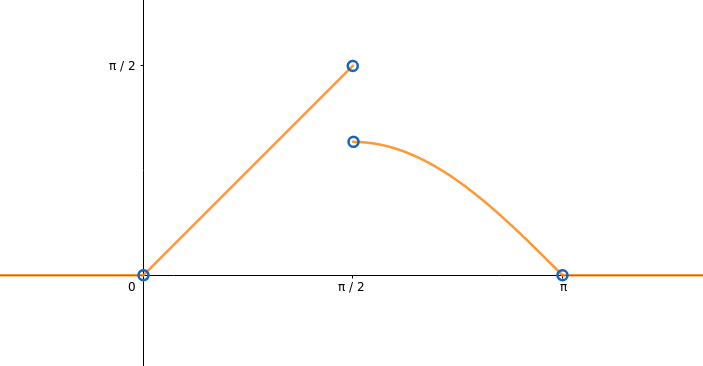
\includegraphics[width=0.9\textwidth]{oef2_heaviside}
\end{center}
}

\item{ \exercise{Gegeven de grafiek van de functie $h(t)$. Bepaal het voorschrift van $h(t)$ en druk uit a.d.h.v. de Heaviside functie.
\begin{center}
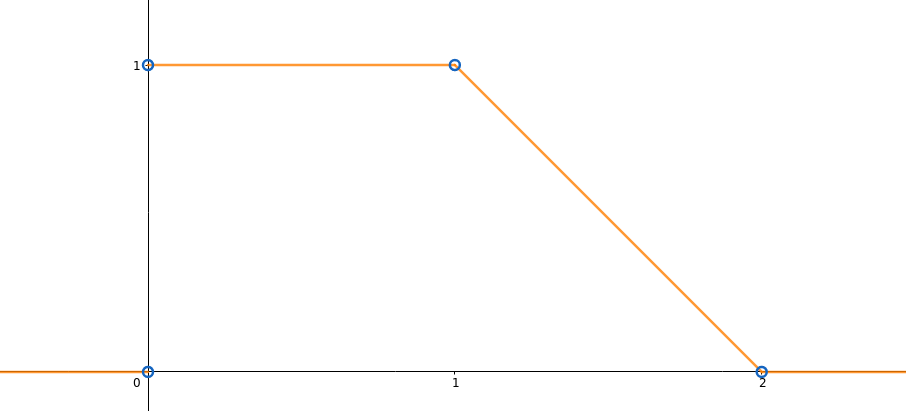
\includegraphics[width=0.9\textwidth]{oef3_heaviside}
\end{center}}{
De functie kan geschreven worden als:
$$h(t) = \begin{cases}
        0 & t < 0 \\
        1 & 0 < t < 1 \\
        2 - t & 1 < t < 2 \\
        0 & t > 2
        \end{cases}
$$
Hieruit volgt gemakkelijk de Heaviside versie hiervan:
\begin{equation*}
\begin{split}
h(t) & = H(t)(-0 + 1) + H(t - 1)(-1 + (2 - t)) + H(t-2)(-(2-t) + 0) \\
    & = H(t) + H(t-1)(1 - t) + H(t- 2)(t - 2)
\end{split}
\end{equation*}}}
\item{
    \exercise{
        Teken de functie $f(t) = 1 + H(t-1)(e^{t}-1) + H(t-2)(2-e^{t})$
    }{
        $$f(t) = \begin{cases}
                    1   & t < 1     \\
                    e^t & 0 < t < 1 \\
                    2   & 1 < t < 2
                 \end{cases}
        $$
        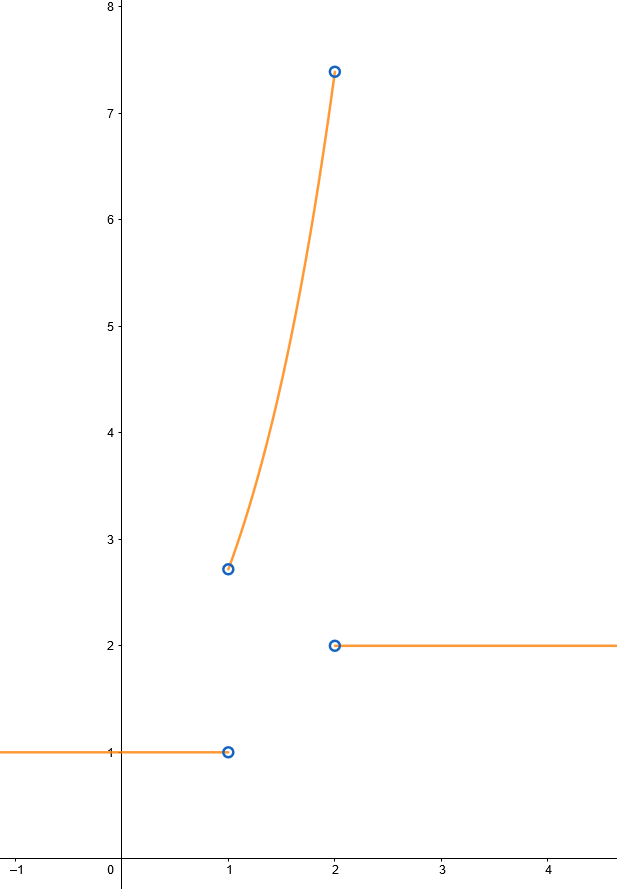
\includegraphics[width=0.9\textwidth]{oef4_heaviside}
    }
}
\end{itemize}
\section{Functies van de exponentiële orde}
\begin{itemize}[label={}]
 \item{
    \exercise{
            Geef de exponentiële orde van $f(t) = te^{-2t}$
    }{
            \begin{equation*}
             \begin{split}
              \lim_{t \to +\infty} \frac{|te^{-2t}|}{e^{\alpha t}} & = \lim_{t \to +\infty} \frac{te^{-2t}}{e^{\alpha t}} \\
                                                                   & = \lim_{t \to +\infty} \frac{t}{e^{\alpha t}e^{2t}}  \\
                                                                   & = \lim_{t \to +\infty} \frac{t}{e^{t(\alpha + 2)}}   \\
                                                                   & \stackrel{H}{=} \lim_{t \to +\infty} \frac{1}{e^{t(\alpha + 2)}(\alpha + 2)} \qquad \hbox{voor}\; \alpha + 2 > 0 \\
                                                                   & = 0 \in \mathbb{R}
             \end{split}
            \end{equation*}
            Dus
            \begin{equation*}
             \begin{split}
                              & \alpha + 2 > 0 \\
              \Leftrightarrow & \alpha > -2
             \end{split}
            \end{equation*}
            De exponentiële orde is -2.
        }}
 \item{
    \exercise{
        Geef de exponentiële orde van $f(t) = 6e^{3t}$
    }{
        \begin{equation*}
         \begin{split}
          \lim_{t \to +\infty} \frac{|6e^{3t}|}{e^{\alpha t}} & = \lim_{t \to +\infty} \frac{6e^{3t}}{e^{\alpha t}} \\
                                                              & = 6\lim_{t \to +\infty} e^{t(3 - \alpha)} \\                                                    
         \end{split}
        \end{equation*}
        Indien $ 3 - \alpha < 0$ dan wordt de limiet 0. De exponentiële orde is dus 3.
    }
 
 }
\end{itemize}
\section{Laplacebeeld}
Bepaal het Laplacebeeld van volgende functies:
\begin{itemize}[label={}]
 \item{
    \exercise{
        $f(t) = 3e^{2t} + t^2 - 5\cos 2t + 4\sin 3t$
    }{
        \begin{equation*}
         \begin{split}
          \mathcal{L}\{3e^{2t} + t^2 - 5\cos 2t + 4\sin 3t\}(s) = \frac{3}{s - 2} + \frac{2}{s^3} - \frac{5s}{s^2 + 4} + \frac{12}{s^2 + 9}
         \end{split}
        \end{equation*}
    }
 }
 \item{
    \exercise{
        $f(t) = (1 + e^{-4t})^2$
    }{
        \begin{equation*}
         \begin{split}
          \mathcal{L}\{(1 + e^{-4t})^2\}(s) & = \mathcal{L}\{1 + 2e^{-4t} + e^{-8t}\}(s) \\
                                            & = \frac{1}{s} + \frac{2}{s + 4} + \frac{1}{s + 8}
         \end{split}
        \end{equation*}
    }
 }
 \item{
    \exercise{
        $f(t) = \sin^2 t$
    }{
        \begin{equation*}
         \begin{split}
          \mathcal{L}\{\sin^2 t\}(s) & = \mathcal{L}\{\frac{1 - \cos 2t}{2}\}(s) \\
                                     & = \frac{1}{2}\mathcal{L}\{1 - \cos 2t\} \\
                                     & = \frac{1}{2}\bigg[\frac{1}{s} - \frac{s}{s^2 + 4}\bigg]
         \end{split}
        \end{equation*}
    }
 }
 \item{
    \exercise{
        $f(t) = t^2\delta(t - 2)$
    }{
        \begin{equation*}
         \begin{split}
          \mathcal{L}\{t^2\delta(t - 2)\}(s) & = \int_{0}^{+\infty} t^2\delta(t-2)e^{-st}\;dt \\
                                             & = [t^2e^{-st}]_{t = 2} \\
                                             & = 4e^{-2s}
         \end{split}
        \end{equation*}
    }
 }
 \item{
    \exercise{
        $f(t) = (t - 1)H(t - 1)$
    }{
        \begin{equation*}
         \begin{split}
          \mathcal{L}\{(t - 1)H(t - 1\}(s) & = e^{-s}\mathcal{L}\{u\}(s) \\
                                           & = \frac{e^{-s}}{s^2}
         \end{split}
        \end{equation*}
    }
 }
 \item{
    \exercise{
        $f(t) = t^2H(t-1)$
    }{
        \begin{equation*}
         \begin{split}
          \mathcal{L}\{t^2H(t-1)\}(s) & = \mathcal{L}\{[(t-1)+1]^2H(t-1)\}(s) \\
                                      & = \mathcal{L}\{(t-1)^2 + 2(t-1)+1)H(t-1)\}(s) \\
                                      & = e^{-s}\mathcal{L}\{u^2 + 2u + 1\} \\
                                      & = e^{-s}\bigg(\frac{2}{s^3} + \frac{2}{s} + \frac{1}{s}\bigg)
         \end{split}
        \end{equation*}
    }
 }
 \item{
    \exercise{
        $f(t) = t^2H(t-1)$
    }{
        \begin{equation*}
         \begin{split}
          \mathcal{L}\{t^2H(t-1)\}(s) & = \mathcal{L}\{[(t-1)+1]^2H(t-1)\}(s) \\
                                      & = \mathcal{L}\{(t-1)^2 + 2(t-1)+1)H(t-1)\}(s) \\
                                      & = e^{-s}\mathcal{L}\{u^2 + 2u + 1\} \\
                                      & = e^{-s}\bigg(\frac{2}{s^3} + \frac{2}{s} + \frac{1}{s}\bigg)
         \end{split}
        \end{equation*}
    }
 }
 \item{
    \exercise{
        $f(t) = \sin(t)H(t-2)$
    }{
        \begin{equation*}
         \begin{split}
          \mathcal{L}\{\sin(t)H(t-2)\}(s) & = \mathcal{L}\{\sin((t - 2) + 2)H(t-2)\}(s) \\
                                          & = \mathcal{L}\{[\sin(t-2)\cos(2) + \cos(t-2)\sin(2)]H(t-2)\}(s) \\
                                          & = \mathcal{L}\{[\sin(t-2)\cos(2) + \cos(t-2)\sin(2)]H(t-2)\}(s) \\
                                          & = e^{-2s}[\cos(2)\mathcal{L}\{\sin(u)\} + \sin(2)\mathcal{L}\{\cos(u)\}(s)] \\
                                          & = e^{-2s}\bigg(\frac{\cos(2)}{s^2+1} + \frac{\sin(2)s}{s^2 + 1}\bigg)
         \end{split}
        \end{equation*}
    }
 }
 \item{
    \exercise{
        $f(t) = t^2e^{-2t}$
    }{
        \begin{equation*}
         \begin{split}
          \mathcal{L}\{t^2e^{-2t}\}(s) & = \mathcal{L}\{t^2\}(s + 2) \\
                                       & = \frac{2}{(s+2)^3}
         \end{split}
        \end{equation*}
    }
 }
 \item{
    \exercise{
        $f(t) = e^t\cos 3t$
    }{
        \begin{equation*}
         \begin{split}
          \mathcal{L}\{e^t\cos 3t\}(s) & = \mathcal{L}\{\cos 3t\}(s - 1) \\
                                       & = \frac{s - 1}{(s - 1)^2 + 9} 
         \end{split}
        \end{equation*}
    }
 }
 \item{
    \exercise{
        $f(t) = e^{-2t}\sin 2t$
    }{
        \begin{equation*}
         \begin{split}
          \mathcal{L}\{e^{-2t}\sin 2t\}(s) & = \mathcal{L}\{\sin 2t\}(s + 2) \\
                                       & = \frac{2}{(s + 2)^2 + 4}
         \end{split}
        \end{equation*}
    }
 }
 \item{
    \exercise{
        $f(t) = t\cos t$
    }{
        \begin{equation*}
         \begin{split}
          \mathcal{L}\{t\cos t\}(s) & = (-1)^1 \frac{d\bigg[\mathcal{L}\{\cos t\}(s)\bigg]}{ds} \\
                                    & = - \frac{d[\frac{s}{s^2 + 1}]}{ds} \\
                                    & = -\frac{(s^2 + 1) - s(2s)}{(s^2 + 1)^2} \\
                                    & = -\frac{s^2 + 1 - 2s^2}{(s^2 + 1)^2} \\
                                    & = \frac{s^2 - 1}{(s^2 + 1)^2}
         \end{split}
        \end{equation*}
    }
 }
 
 \item{
    \exercise{
        $f(t) = e^{-2t}t\cos^2 \frac{t}{2}$
    }{
        \begin{equation*}
         \begin{split}
          \mathcal{L}\{e^{-2t}t\cos^2 \frac{t}{2}\}(s) & = \mathcal{L}\{t\cos^2 \frac{t}{2}\}(s + 2) \\
                                                       & = \mathcal{L}\bigg\{t\frac{1 + \cos t}{2}\bigg\}(s + 2) \\
                                                       & = \frac{1}{2}\bigg(\mathcal{L}\{t\}(s + 2) + \mathcal{L}\{t \cos t\}(s+2)\bigg) \\
                                                       & = \frac{1}{2}\bigg(\frac{1}{(s+2)^2} + \frac{(s+2)^2 - 1}{((s+2)^2 + 1)^2}\bigg) \\
         \end{split}
        \end{equation*}
    }
 }
 \item{
    \exercise{
        $f(t) = e^{-3t}t^3H(t - 2)$
    }{
        \begin{equation*}
         \begin{split}
          \mathcal{L}\{e^{-3t}t^3H(t - 2)\}(s) & = \mathcal{L}\{t^3H(t - 2)\}(s + 3) \\
                                               & = \mathcal{L}\{[(t-2)+2]^3H(t-2)\}(s + 3) \\
                                               & = \mathcal{L}\{[(t-2)^3 + 6(t-2)^2+12(t-2) + 8]H(t-2)\}(s + 3) \\
                                               & = e^{2s}\mathcal{L}\{u^3 + 6u^2 + 12u + 8\}(s + 3) \\
                                               & = e^{2s}\bigg[\frac{3!}{(s+3)^4}+6\frac{2!}{(s+3)^3}+12\frac{1!}{(s+3)^2} + 8\frac{1}{s}\bigg] \\
                                               & = e^{2s}\bigg[\frac{6}{(s+3)^4}+\frac{12}{(s+3)^3}+\frac{12}{(s+3)^2} + \frac{8}{s}\bigg] \\
                                               & = 2e^{2s}\bigg[\frac{3}{(s+3)^4}+\frac{6}{(s+3)^3}+\frac{6}{(s+3)^2} + \frac{4}{s}\bigg]
         \end{split}
        \end{equation*}
    }
 }
 \item{
    \exercise{
        $f(t) = \begin{cases}
                 \cos 2t & 0 < t < \frac{\pi}{4} \\
                 e^{2t}t & t > \frac{\pi}{4}
                \end{cases}$

    }{
        \begin{equation*}
         \begin{split}
          f(t) & = \cos 2t + H\big(t-\frac{\pi}{4}\big)(-\cos 2t + e^{2t}t) \\
               & = \cos 2t + (e^{2t}t - \cos 2t)H\big(t - \frac{\pi}{4}\big) \\
          \mathcal{L}\{f(t)\}(s) & = \mathcal{L}\{\cos 2t\}(s) + \mathcal{L}\{e^{2t}tH\big(t - \frac{\pi}{4}\big)\}(s) - \mathcal{L}\{\cos(2t)H\big(t - \frac{\pi}{4}\big)\}(s)
         \end{split}
        \end{equation*}
    We lossen deze 3 Laplacetransformaties individueel op
    \begin{enumerate}
     \item \begin{equation*}
            \begin{split}
                \mathcal{L}\{\cos 2t\}(s) = \frac{s}{s^2 + 4}
            \end{split}
           \end{equation*}
     \item \begin{equation*}
            \begin{split}
                    \mathcal{L}\{e^{2t}tH\big(t - \frac{\pi}{4}\big)\}(s) & = \mathcal{L}\{tH\big(t - \frac{\pi}{4}\big)\}(s - 2) \\
                                                                        & = \mathcal{L}\{\big(t - \frac{\pi}{4} + \frac{\pi}{4}\big)H\big(t - \frac{\pi}{4}\big)\}(s - 2) \\
                                                                        & = e^{-\frac{\pi}{4}s}\mathcal{L}\{\big(u + \frac{\pi}{4}\big)\}(s - 2) \\
                                                                        & = e^{-\frac{\pi}{4}s}\bigg(\frac{1}{(s - 2)^2} +  \frac{\pi}{4(s - 2)}\bigg)
              \end{split}
             \end{equation*}
    \item \begin{equation*}
            \begin{split}
                \mathcal{L}\{\cos 2t\;H\big(t - \frac{\pi}{4}\big)\}(s) & = \mathcal{L}\{\cos \big[2\big(t-\frac{\pi}{4} + \frac{\pi}{4}\big)\big]H\big(t - \frac{\pi}{4}\big)\}(s) \\
                                                                        & = \mathcal{L}\{\cos\big[2\big(t - \frac{\pi}{4}\big) + \frac{\pi}{2}\big]H\big(t - \frac{\pi}{4}\big)\}(s) \\
                                                                        & = \mathcal{L}\{[\cos 2(t - \frac{\pi}{4})\cos\frac{\pi}{2} - \sin 2(t - \frac{\pi}{4})\sin\frac{\pi}{2}]H\big(t - \frac{\pi}{4})\}(s) \\
                                                                        & = - \mathcal{L}\{\sin 2(t - \frac{\pi}{4})H(t - \frac{\pi}{4}\}(s) \\
                                                                        & = e^{-\frac{\pi}{4}s}\mathcal{L}\{\sin 2u\} \\
                                                                        & = \frac{2e^{-\frac{\pi}{4}s}}{s^2 + 4}
            \end{split}
           \end{equation*}
    \end{enumerate}
    Uiteindelijk:
    $$\mathcal{L}\{f(t)\}(s) = \frac{s}{s^2 + 4} + e^{-\frac{\pi}{4}s}\bigg(\frac{1}{(s - 2)^2} +  \frac{\pi}{4(s - 2)}\bigg) - \frac{2e^{-\frac{\pi}{4}s}}{s^2 + 4}$$
    }
 }
 
 
\end{itemize}

\section{Invers Laplacebeeld}
Bepaal het invers laplacebeeld van volgende functies:
\begin{itemize}[label={}]
 \item{
    \exercise{
        $f(s) = \frac{1}{s^3}$
    }{
        \begin{equation*}
         \begin{split}
          \mathcal{L}^{-1}\bigg\{\frac{1}{s^3}\bigg\}(t) & = \frac{1}{2!}\mathcal{L}^{-1}\bigg\{\frac{2!}{s^3}\bigg\}(t) \\
                                                         & = \frac{t^2}{2}
         \end{split}
        \end{equation*}
    }
 }
 \item{
    \exercise{
        $f(s) = \frac{s + 5}{s^4}$
    }{
        \begin{equation*}
         \begin{split}
          \mathcal{L}^{-1}\bigg\{\frac{s + 5}{s^4}\bigg\}(t) & = \mathcal{L}^{-1}\bigg\{\frac{s}{s^4} + \frac{5}{s^4}\bigg\}(t) \\
                                                             & = \mathcal{L}^{-1}\bigg\{\frac{1}{s^3}\bigg\}(t) + 5\mathcal{L}^{-1}\bigg\{\frac{5}{s^4}\bigg\}(t) \\
                                                             & = \frac{1}{2!}\mathcal{L}^{-1}\bigg\{\frac{2!}{s^3}\bigg\}(t) + \frac{5}{3!}\mathcal{L}^{-1}\bigg\{\frac{3!}{s^4}\bigg\}(t) \\
                                                             & = \frac{t^2}{2} + \frac{5t^3}{6}
         \end{split}
        \end{equation*}
    }
 }
 \item{
    \exercise{
        $f(s) = \frac{1}{3s - 1}$
    }{
        \begin{equation*}
         \begin{split}
          \mathcal{L}^{-1}\bigg\{\frac{1}{3s - 1}\bigg\}(t) & = \frac{1}{3}\mathcal{L}^{-1}\bigg\{\frac{1}{s - \frac{1}{3}}\bigg\}(t) \\
                                                            & = \frac{1}{3}e^{\frac{1}{3}t} \\
                                                            & = \frac{1}{3}e^{\frac{t}{3}}
         \end{split}
        \end{equation*}
    }
 }
 \item{
    \exercise{
        $f(s) = \frac{2s + 3}{s^2 - 5s + 6}$
    }{
        \begin{equation*}
         \begin{split}
          \mathcal{L}^{-1}\bigg\{\frac{2s + 3}{s^2 - 5s + 6}\bigg\}(t) & = \mathcal{L}^{-1}\bigg\{\frac{2s + 3}{(s-2)(s-3)}\bigg\}(t) \\
          \Rightarrow & \frac{2s + 3}{(s-2)(s-3)} = \frac{a}{s - 2} + \frac{b}{s-3} = \frac{a(s-3) + b(s-2)}{(s-2)(s-3)} \\
          \Rightarrow & 2s + 3 = a(s-3) + b(s-2) \Rightarrow \begin{cases}
                                                              a = -7 \\
                                                              b = 9
                                                             \end{cases} \\
                                                             & =  \mathcal{L}^{-1}\bigg\{\frac{-7}{s - 2} + \frac{9}{s - 3}\bigg\}(t) \\
                                                             & = -7e^{2t} + 9e^{3t}
         \end{split}
        \end{equation*}
    }
 }
 \item{
    \exercise{
        $f(s) = \frac{4s + 3}{s^2 + 16}$
    }{
        \begin{equation*}
         \begin{split}
          \mathcal{L}^{-1}\bigg\{\frac{4s + 3}{s^2 + 16}\bigg\}(t) & = \mathcal{L}^{-1}\bigg\{\frac{4s}{s^2 + 16} + \frac{3}{s^2 + 16}\bigg\}(t) \\
          & = 4\cos 4t + \frac{3}{4}\sin 4t
         \end{split}
        \end{equation*}
    }
 }
 \item{
    \exercise{
        $f(s) = \frac{s + 3}{s(s^2 + 9)}$
    }{
        \begin{equation*}
         \begin{split}
          \mathcal{L}^{-1}\bigg\{\frac{s + 3}{s(s^2 + 9)}\bigg\}(t) \\
          \Rightarrow & \frac{s + 3}{s(s^2 + 9)} = \frac{a}{s} + \frac{b + cs}{s^2 + 9} = \frac{a(s^2 + 9) + (b+cs)s}{s(s^2 + 9)} \\
          \Rightarrow & s + 3 = a(s^2 + 9) + (b + cs)s \Rightarrow \begin{cases}
                                                                    a = \frac{1}{3} \\
                                                                    b = -\frac{1}{3} \\
                                                                    c = 1
                                                                   \end{cases} \\
                    & = \mathcal{L}^{-1}\bigg\{\frac{1}{3s} \bigg\} + \mathcal{L}^{-1}\bigg\{\frac{-\frac{1}{3}}{s^2 + 9} \bigg\} + \mathcal{L}^{-1}\bigg\{\frac{s}{s^2 + 9} \bigg\} \\
                    & = \frac{1}{3} - \frac{1}{3}\cdot\frac{1}{3}\mathcal{L}^{-1}\bigg\{\frac{3}{s^2 + 9}\bigg\} + \cos 3t \\
                    & = \frac{1}{3} - \frac{1}{9}\sin 3t + \cos 3t
         \end{split}
        \end{equation*}
    }
 }
\end{itemize}




\end{document}

